%!TeX root = ./../MusterAbschlussarbeit.tex

%##########################################################
% Inhalt
%##########################################################
\clearpage
\chapter{Konzeption}

\section{Das Würfelspiel: Noch Mal}
Im modellierten Spiel 'Noch Mal!' geht es darum so viele Kästchen anzukreuzen und möglichst viele Spalten und gleichfarbige Kästchen auszufüllen.
Farb und Zahlenwürfel müssen kombiniert werden um entsprechend zusammenhängende Felder der gewählten Farbe abzukreuzen.

\subsection{Spielablauf Einspieler Variante}
Der Spieler Würfelt alle 4 Würfel bestehend aus 2 Farb und 2 Zahlenwürfeln.
Der Spieler hat 30 Züge dazu Zeit maximale Punkte zu erreichen.
Anschließend wählt er ein paar aus Farb- und Zahlenwürfel aus und kreuzt entsprechend des gewürfelten Paares verfügbare Felder auf dem Spielfeld ab.
Ein Spieler darf immer entscheiden ob er Würfelwürfe zum ankreuzen verwenden möchte oder nicht.
Um Kästchen anzukreuzen, wählt der Spieler eine Kombination aus Zahlen bzw Farbwürfel aus. Wählt er Beispielsweise 'Grün' und '2' so müssen 2 zusammenhängende Grüne Felder angekreuzt werden.


\newpage
\subsection{Spielregeln}
\setlist{noitemsep}
\begin{enumerate}
    \item Felder in der Spalte H sind von Beginn an verfügbar
    \item Alle Kreuze müssen immer zusammenhängend in genau einem Farbblock der gewählten Farbe platziert werden
    \item Kreuze müssen waagerecht oder senkrecht benachbart zu einem bereits abgekreuzten Feld oder Teil der Spalte H sein um verfügbar zu werden
    \item Es müssen genau so viele Felder angekreuzt werden wie das Ergebnis des gewählten Zahlenwürfels
    \item Es könnte nicht mehr als 5 Kästchen in einem Zug abgekreuzt werden
    \item Wird ein Zahlenjoker gewählt, darf der Spieler eine Zahl von 1-5 bestimmen
    \item Wird ein Farbjoker gewählt, darf der Spieler eine Farbe bestimmen
\end{enumerate}

\subsection{Optimale Spielstrategie}
Um im Spiel 'Noch mal' eine möglichst hohe Anzahl an Punkten zu erhalten, ist es wichtig nach folgenden Strategien zu spielen:
\setlist{noitemsep}
\begin{enumerate}
    \item \textbf{Priorisierung äußerer Spalten}: Äußere Spalten geben mehr Punkte, weshalb es wichtig ist diese komplett auszufüllen.
    \item \textbf{Beenden von Farben}: Vollständig ausgefüllte Farben geben viele Extrapunkte. Im späten Spielverlauf kann es besser sein Farben komplett zu füllen anstatt Spalten zu werten.
    \item \textbf{Priorisieren von Sternfeldern}: Jedes ausgefüllte Sternfeld gibt 2 Punkte, eine gute Spielweise ist es so viele Sternfelder wie möglich auszufüllen.
    \item \textbf{Strategische Nutzung von Jokern}: Ungenutzte Joker geben zum Ende des Spiels Punkte. Es ist gut diese so wenig wie möglich zu nutzen um Extrapunkte zu bekommen. Jedoch können mit Hilfe von Jokern einfach bestimmte Felder gewählt werden, welche benötigt werden um eine Wertung zu erzielen.
\end{enumerate}

\subsection{Punktevergabe}
Gelingt es dem  Spieler eine Spalte komplett auszufüllen, erhält er je nach Spalte Punkte dafür. Äußere Spalten mehr Punkte vergeben werden als für die inneren Spalten.
Für das komplette Ausfüllen einer Farbe erhält der Spieler fünf Punkte pro ausgefüllter Farbe.
Jedes nicht angekreuzte Sternfeld gibt zum Spielende zwei Minuspunkte.
Für jeden übrig gebliebenen Joker erhält der Spieler zum ende des Spiels einen Punkt.
\begin{figure}[!h]
	\centering
	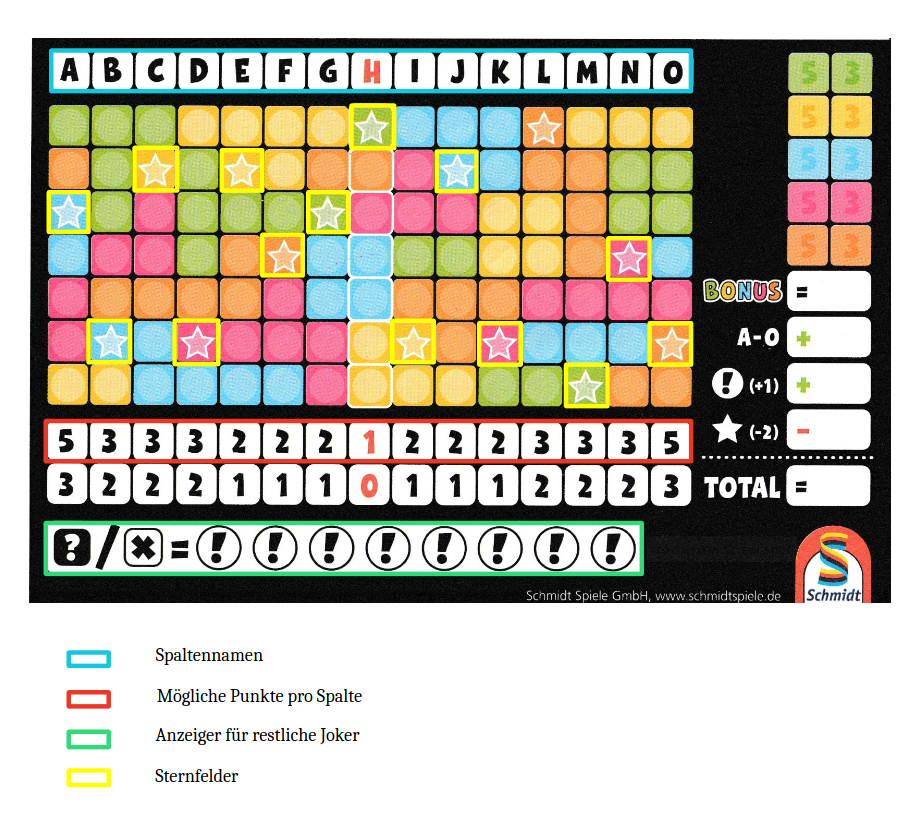
\includegraphics[width=0.5\textwidth]{Bilder/Abbildung2.png}
	\caption{Quelle: Aus Noch mal! von Schmidt Spiele, Grafik zur Erklärung der Punktevergabe}
\end{figure}

\begin{figure}[!h]
	\centering
	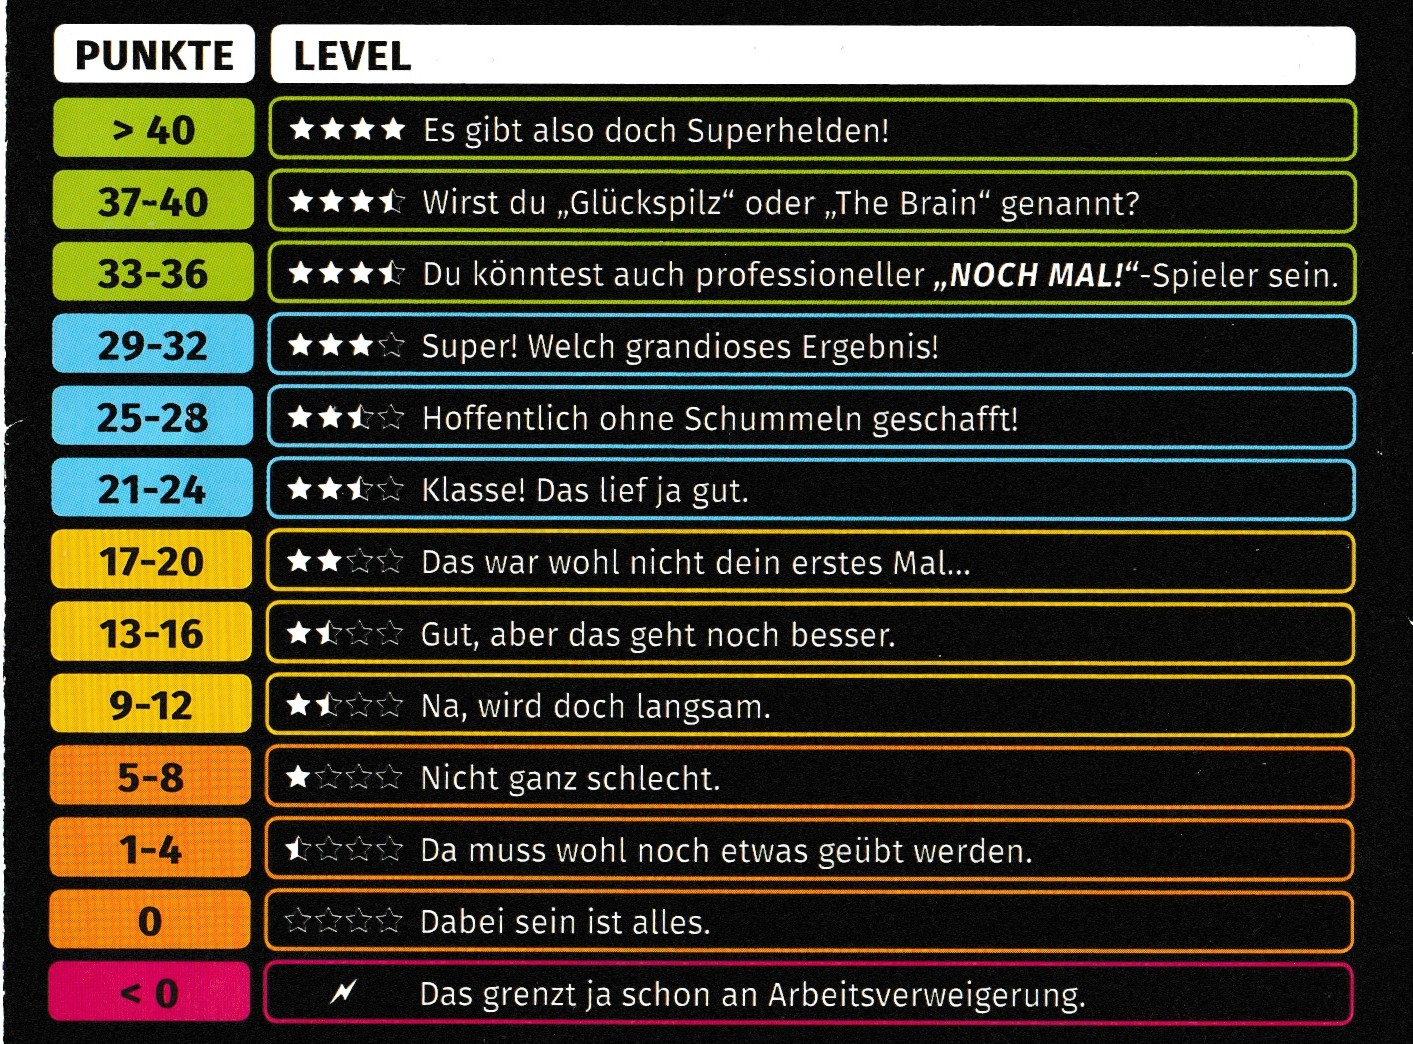
\includegraphics[width=0.5\textwidth]{Bilder/Punkte.jpeg}
	\caption{Quelle: Aus Noch mal! von Schmidt Spiele, Grafik zur Bewertung der gesammelten Punkte der Einspieler Variante}
\end{figure}
\newpage

\section{Vorgehensweise}
Gehört das hier tatsächlich hin?
Und wenn ja was soltle dewn nhjier bittte rein?
